\documentclass[a4paper,12pt,twoside]{ltxdoc}

%\usepackage[utf8]{inputenc} % not used, as I compile with Xelatex
\usepackage[T1]{fontenc}
\usepackage[english]{babel} % Language, could be set to swedish
\usepackage{fancyhdr} % Header and footers
\usepackage{verbatim} % Better Verbatim packages
\usepackage{fancyvrb}
\usepackage{amssymb,amsmath}
\usepackage{graphicx} % PNG and SVG images, and such.
\usepackage{enumerate} % better listing options
\usepackage{hyperref} % URL and stuff.
\usepackage[margin=2.5cm]{geometry}

\pagestyle{fancy}

\fancyhead[LH]{Group 11}
\fancyhead[RH]{Sentiment Analysis in Speech with Relation to Brands}
%\fancyfoot[LO]{\thepage}
%\fancyfoot[RE]{\thepage}
\title{Project: Search Engines and Information Retrieval Systems}
\author{
Jens Arvidsson <\href{mailto:jensarv@gmail.com}{jensarv@gmail.com}> \and
Fredrick Chahine <\href{mailto:fchahine@kth.se}{fchahine@kth.se}> \and
Erik Hallström  <\href{mailto:erik_hallstrom@icloud.com}{erik\_hallstrom@icloud.com}> \and
Petter Salminen <\href{mailto:petsal@kth.se}{petsal@kth.se}>}


\newcommand*\sepline{%
  \begin{center}
    \rule[1ex]{.5\textwidth}{.5pt}
  \end{center}}

% Kodkommando
\newcommand{\javafil}[1]{\lstinputlisting{#1}} % #1 = filnamn, #2 = caption
\newcommand{\ovning}[1]{\section*{Övning #1}}

\begin{document}
\maketitle
\tableofcontents

%\listoffigures
%\listoftables
\newpage
\begin{abstract}
In the following project we made a program that does a \emph{Sentiment Analysis} for a given brand on one of the following three things: A live recording using the microphone. A folder containing several audio files. A string inserted into the text box.

This because our client, Jussi at Gavagai, wants us to try out if it is possible to develop a platform that can perform Sentiment Analysis for brands given that the input data is in the form of a audio file, since there is no known platform to perform just this. 

Using an \verb#API# given to us by Jussi, the program grades the given input on the five given levels: Sexy, Violence, Positive, Negative and Uncertainty. 

For example, the given input of ``When I drink coca cola I feel super good and it makes me smile so much yeah coca cola is my favorite drink'' tells us that coca cola in this sentence is seen in a positive way. 

When the speech-to-text \verb#API# works great, our program works like a charm, and is very good for catching the general attitude towards a given brand. But the text to speech \verb#API# we're using is quite crude. This means that in many of our test cases gives it gave us very weird (non logical text) from the given vocal input. When this happens our program will also give very bad results, especially when the brand itself disappears from the text.

The least we can say that we're very happy with the results. And hope that our client will be happy with our experimental results.
\end{abstract}

\section{Contributions}
\subsection{Jens}
Jens has written the basic interface code and the code communicating with/parsing replies from both of the API servers, as well as carrying out the experiments and writing the Results section of the report.


\subsection(Fredrick)
Fredrick started out by researching text-to-speech analysis tools. He wrote the Background and Method sections of the report.

\subsection{Erik}
Erik has written the code for inputing brands and search for mentions of them in the text, recording and converting file formats and presenting the results in the table. In the report he wrote the section about previous work in text-to-speech and the discussion.




\subsection{Petter}
Petter has done much on the report, mostly \LaTeX things to make this document look acceptable. But when it comes to writing he wrote the Abstract, Sentiment Analysis and small parts of the Text-to-Speech.  Also, he has done all the posters for the poster session. In the beginning he tried to find audio files (with brands in them) to analyze, and also record some of his own.

\newpage
\section{Background}
Today, we have more ways than ever of sharing information thanks to the Internet and social media. We can share our
thoughts, feelings, and experiences with just a few button strokes. In addition, consumers today can reach a wide audience
when they express their feelings about products and brands. This data on consumer preferences is of great value to companies.
Companies can mine the data to extract trends and opinions from their clients. And yet, there is an oasis of spoken
data relating to this area that remains unexploited.

At the same time, technology is moving forward multiple levels. Portable devices are capable of recording better quality
audio than they were ten years ago. Smartphones are also far more ubiquitous than they were at the time.
Furthermore, new \verb#API#s are emerging that make it easy to process audio recordings. These technological advancements herald
in opportunities that are of great value to companies. The possibility to effectively process live or recorded audio
to elicit consumer thoughts and preferences may be just around the corner. Empowered with this information, companies will
be able to position their product lines accordingly.

And yet, there are some unresolved issues. Data may be difficult to process for several reasons. One reason is the sheer
amount of it. Another aspect of information that may make it difficult to process is its format. The spoken word can be 
far more difficult to process that a written document. To capitalize on this treasure trove of information, we need
to develop effective ways of deriving details from the spoken word and processing them.

With most of our media still being partly or fully in form of sound, such as web radio, and television.
It is hard to analyze all the information being run around on this media, as the format is not
native to our computers and systems. 

With this is mind, our mission is to make an experimental program that can transcribe speech and analyze it, looking for certain trends.
For example, this can be used to recognize branding recognition from a audio stream, and then analyze the context to find an opinion about the brand.
A complete solution could be very interesting for companies who care to know how their brand is doing ``out there'' in the world.

\section{Related Work}
\subsection{Speech-to-Text}
\emph{Speech-to-text}, or more generally \emph{Computer Speech Recognition} is the general problem in computer science where the computer has to translate spoken words into text.

The first real attempt to do speech recognition was made during the 50's and the system could only handle a small subset of speech, namely digit recognition. In 1952 researchers at Bell Laboratories built a speech recognition system that only could recognize digits by a single speaker in a quiet room. The technology of  the system was based on the theory of the acoustics of speech and the machine triggered on the sound of the vowels in the different digits.

Similar work was made by researchers at RCA Laboratories and at MIT Lincoln Lab during the 50's. The research teams at these two institutions built speech recognition systems that could classify vowels that a test person spoke.

Moving on to the 60's, there were several Japanese teams that had progress with speech recognition, especially two professors named Suzuki and Nakata at Kyoto University. Even though they still only could recognize single digits or vowels, however the difference here was that these could be recognized in continuous speech. The earlier systems assumed each utterance of the test speaker contained the complete digit or vowel and thus did not need to be actively segmented.  

During the 70's the first speech recognition system that could handle spoken words an sentences began to be developed. A program named "Harpy" was made at Carnegie Mellon University and could recognize speech containing 1011 different words. It had a moderate performance. Harpy used a graph search algorithm to obtain the results. 

A new technology based on the n-gram language model, was introduced in the beginning of the 80's and have been very important to speech recognition systems ever since. One obvious task for a speech recognizer is to use it as a automatic typewriter; a user speaks words and sentences that should be written to a document. Since there is an underlying structure and grammar in all form of language, not all letter orderings and word orderings are equally probable. In fact, some orderings are even wrong, i.e the words are misspelled or sentences are grammatically incorrect. The n-gram model looks at a sequence of words and tells how probable it is. That will help when doing the word recognition, we will get a prior for each word and thus use a \verb#M.A.P# estimation for what the next word ought to be.

These typewriters was suppose to be used extensively by certain persons, thus they allowed for individual training of the system. This was not the case for another application of speech recognition, namely routing phone-calls. Usually when calling support centers there is a need for routing phone-calls to the correct expert or department. This require a large workforce of operators and if it could be automated the companies could save a lot of money. These systems where to be used on demand by millions of people, thus they needed to generalize very well among different voices and regional accents. The utilization of this technology started in the early 90's and today such systems are annually routing billions of phone calls around the world. 

A technology that was developed and became more prevalent during mid 80's was the hidden Markov model (\verb#HMM#). It quickly became the best and most preferred method for speech recognition. In a hidden Markov model, state and observation are key concepts. States are what the actual quantity being estimated is equal to. The obvious choice is words, but there are modified models and other quantities could be chosen to represent the states. The HMM models the state transitions between the words based on uncertain measurements and the probability of a new word given the previous word. The state transitions have certain probabilities and some transitions are more probable than others that might result in bad grammar or weird sentences.  The measurements are the speech itself, sound waves captured from the microphone\cite{history}.

Further on more modern machine learning techniques such as support vector machines and artificial neural networks has been used to get promising results within the field.

Today the use of speech-to-text or speech recognition can be found in many different fields and applications. It is extensively used in industry and by customers. Hands-free computing; writing emails just by talking to the computer, voice recognition on the cellphone to determine whom to call or what music to listen to or perhaps new intelligent assistants such as Apple iPhone's Siri are helping people to do daily tasks with speech recognition. Google uses speech recognition similar to Siri on their Android phones, but also as text input to their search engine with together with Google Chrome. This is the service we are using in our program.


%% Text about some how speech-to-text works.

\subsection{Sentiment Analysis}
The \emph{Sentiment Analysis} or \emph{Opinion Mining} problem is that given any snippet of text, to find the general attitude of given text on a topic.
As an very simple example, the text ``I hate Mondays'' has a very negative attitude, while the attitude of ``I would not prefer Mondays'' is more towards neutral.

Some early work in the area would be for example to sample reviews of a movie, or restaurant and analyze the polarity of it. Early work on this has been acknowledged to be done by Turney\cite{turney} and Pang\cite{pang}

To be able to get the general opinion or attitude from a text can be very useful for companies that care about their reputation.
Thus for example finding a lot of complains about something could give great automatic feedback.

With extreme rise of social media platforms such as \emph{Twitter} and \emph{Facebook}, the general interest in sentiment analysis has skyrocketed. Businesses look for solutions to automate the data mining of these platforms, analyzing the general opinion and if case getting negative feedback, to be able to immediately attend to the issues.

\section{Method}

Our solution to this problem consists of three steps, which are later combined into a single program.

\begin{enumerate}
\item Our first step is to work convert speech-to-text. For this we use Google's speech \verb#API#.

\item Next, we process the converted text to capture brands that the data miner is interested in.

\item Finally, we process the expressions related to these brands to detect sentiments, using Gavagai's \verb#API#.
\end{enumerate}

Google's speech \verb#API# is used widely across its product range, from web search to translate to Android voice commands.
Provided with an audio file in \verb#FLAC# format, the \verb#API# returns a \verb#JSON# object representing the transcribed audio. The \verb#JSON# object
can then be parsed to retrieve the text string that corresponds to the spoken message. Google's speech \verb#API# allows for a number
of different configuration settings, including language and audio frequency of the supplied file. However, it only allows for file sizes up to 256 kB, 
which means that larger recordings must be split up into smaller parts and submitted individually.

In our project, audio file input is extended by letting the user of the program record an audio snippet in real time and
then submit it for processing.

In the second step, mentions of brands are elicited from the transcribed audio. In our program, the user supplies the name
of a brand that he or she wants to watch for. The user also chooses how many words before an after the brand name should
be included in the analysis. Thus, there is a precision-vs-recall trade-off here. Choosing a large number of words to include
in the processing increase the scope of the search, but might lower the precision as unrelated adjectives may be grouped
with the brand mention.

In the third step, we provide cardinal scores of the audio according to a number of criteria. Gavagai's \verb#API# lets us
evaluate a text string based on a number of parameters. We can look for the sentiments described as positive, negative, sexy, violent,
and uncertain. The program then presents the user with the data tabulated as shown in the figure. %% bild här

\begin{center}
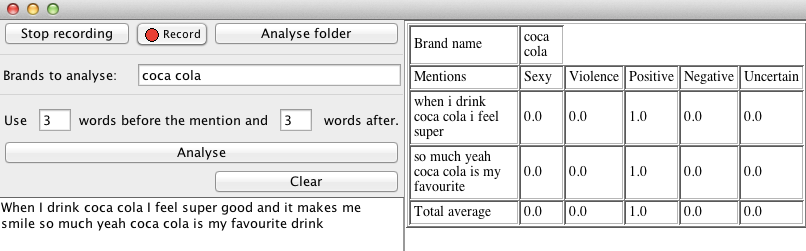
\includegraphics[scale=0.6]{../poster/screenshot_crop.png}
\end{center}

Our solution to this problem consists not of trying to reinvent the wheel, but of employing different
solutions that are more-or-less complete throughout the different stages, and then stitching them together.

First and foremost we have an audio file, which we will send to Google speech \verb#API#, which will give us a fair caption of the given sound segment.

This text we can then search for given brands or other point of interests, and then send this text for textual attitude analyzing using an web \verb#API# provided by our mentor at Gavagai.

From here we will get a score, from which we can show the user what kind of attitude the speech had. 

\section{Results}
The program was tested on a few different scenarios, to measure its performance under different conditions, as well as testing the limits of the frameworks used in it. The tests were done in a 4 step process:

\begin{itemize}
\item Input text into the program and run a sentiment analysis for brands mentioned in it.
\item Record one of the authors reading the text aloud, and input it into the program.
\item Compare the sentiment scores of the text and the audio file.
\item Compare the sentiment scores to the content of the text.
\end{itemize}

\subsection{Big files}
The test text used for this test was a long blog post detailing the authors' love for the Coca-Cola soft drink. The sentiment scores for the text itself indicated that the text was both positive and sexy:
Sexy: 0.42857142857142855 Violent: 0.14285714285714285 Positive: 1.2857142857142858 Negative: 0.07142857142857142


Unfortunately, due to limitations on big files, the output from he speech-to-text \verb#API# was mostly unintelligible, and very little of the original text survived the conversion. Thus, the results were unusable for any sane comparison. This finding limited our testing to small files, and hindered testing on podcasts, live streams and other interesting audio sources.

\subsection{Mixed brands}
In this test, short texts which mention multiple brands with different sentiments were used. The program was configured to use a small scope when searching for sentiments, 3 words behind and 3 words after the brand name. The audio file input was a failure, since most of the time brand names weren't picked up by the speech-to-text \verb#API#, so no sentiment analysis could be done on these texts. Even if the brand names were inserted, differing sentiments in the same text meant that the sentiment analysis often gave bad results. For example, the sentence ``I love Coke, but I hate my Ford. Although, Coke is really nice to drink while driving, so I guess the Ford isn't completely worthless.'', with the score for Coke being 
Sexy: 1.5, Positive: 1.5, Negative:1.0
and the score for Ford being
Negative: 0.5

when read aloud and input through the program became ``I love I need so who is he nice to drink while driving so I guess the board in completely worthless''.

which, aside from seemingly having nothing to do with either Ford or Coca-Cola, gets a general sentiment score of 
Sexy: 2.0, Positive: 2.0, Negative:2.0
Three other, similar text snippets were recorded and tried, and produced similar results not possible to compare with the original text snippets.

\subsection{Small snippets, one brand, one sentiment}
The last test was made to ascertain that our program worked at all as intended, as the examples are idealized and might not be encountered in a real situation. They do, however, overcome the limitations set on our experimental program by the outside services used to power it, and as such serve as an adequate proof of concept. The snippets used are small, they contain only one brand that is mentioned multiple times (Ford), and the whole snippet only contains one sentiment. The scope used was ten words behind, twenty words after.

The results are presented below. First the original text and its sentiment score, and then the processed recording of it being read aloud and the associated sentiment score.

\begin{center}
``I love Ford since they make the best cars I have one myself and it is not only very efficient but also quiet and has a lovely design My friend tipped me off about it and Ive been happy with the car ever since.''
\end{center}
\hfill Score: Sexy: 2.0 Positive: 4.0

\begin{center}
``I love Ford they make the best cars I have one myself only there any fish in it also quite lovely night my friend to pick me up about it and I've been happy with the car.''
\end{center}
\hfill Score: Sexy: 2.0, Positive: 4.0

\sepline

\begin{center}
``My friend just bought a Ford, and I can't say anything about it really. It's a pretty standard car, and I'm unsure about what made him choose it. He's kind of average, so maybe he likes a car that's as mundane as himself.''
\end{center}
\hfill Score: Positive: 1.0, Negative: 1.0, Uncertain: 2.0

\begin{center}
``my friend just bored and I can send about it it's a pretty standard and I'm unsure about with meetings so maybe like the car and a Nazi.''
\end{center}
\hfill Score: Positive: 1.0, Negative: 1.0, Unsure: 2.0

Note: The sentiment analysis for this snippet was run on the whole text since the word ``Ford'' was not picked up, so this snippet would probably not be considered in a larger analysis.

\sepline

\begin{center}
``I can't believe that Ford still exists as a company. They make awful cars, and have a terrible history as one of the worst environment crooks among the big auto companies. Don't buy Fords, people!''
\end{center}
\hfill Score: Negative: 2.0

\begin{center}
``I can't believe the Ford still exist the company they make of a car and have a tear as one of the work environment cooks big auto companies don't buy Ford Depot''
\end{center}
\hfill No sentiments were picked up by the sentiment analysis

\sepline 

\begin{center}
``Some guy just trashed my Ford and beat me up. He somehow punched right through my windshield, threatened by pull my car tires off and then ran away screaming. This day could not get any worse.''
\end{center}
\hfill Score: Violence: 3.0, Uncertain: 1.0

\begin{center}
``oMG I just passed by Ford beat me up he somehow right to my wii ready to pull my car tires off and then run away screen this day could not get any books''
\end{center}
\hfill Score: Violence: 1.0, Uncertain: 1.0

\section{Discussion}
The scope of this project is obviously too small to design our own speech recognition algorithm or sentiment analysis algorithm. We had to rely on 3rd party services such as the speech sentiment API from Gavagai and Googles unofficial speech recognition web service. Even though a large international company like Google uses cutting edge technology for their speech recognition, we had major problems recognizing some of the words, even when the speaker was alone in a quiet room and spoke at normal speed. Especially recognizing the brands themselves proved to be fairly hard. Sometimes only one out of several mentions was recognized, making the end results worse. 

When we first began with this project we tried to use CMU Sphinx, a speech recognition system developed at the Carnegie Mellon University, now open source. However the setup showed to be very cumbersome and we simply didn't manage to make it work. Given the short time schedule we turned to Googles unofficial web service. We figured we would still get as good a result as possible since Google are using the same speech-to-text service in their products. 

The text to speech function did however do well when using short recordings or sound files as opposed to long recordings which did comparatively worse. The reason for this was that we had to break up the sound files into segments of 256 kB and classify them one by one. This had to be done due to Googles own restrictions on large files. If a sentence was broken up just in the middle it sometimes resulted in grammatically incorrect phrases. Since the speech-to-text algorithms are based on grammar this furthermore worsened the speech recognition results.

As for the sentiment analysis it preformed as expected and did fairly well if the text was typed in or pasted by hand. Certainly it performed better the more data that was available, so larger texts producer more precise results. 

The program had the capability to input several brands and do sentiment analysis at the same time on the corpus. When speaking of several brands at the same time in a recording, the algorithm produced very bad results. Firstly the speech recognition is worse when mentioning more special words that can not be put in a grammatically context, and secondly the sentiment analysis doesn't seem to care that much about grammar and order of the words in the input. When doing multiple brand sentiment analysis where the brands where mentioned close to each other they sometimes seemed to be mixed up. 

Our program did produce reasonable results when just mentioning one brand in a short sound file with the same sentiment towards the brand all along the conversation. 

\newpage 

%% Here is the ref system, where you add an item
%% as you can see with the \bibitem{NAME} field.
%%
%% To in the text refer to a certain reference, use
%% this command \cite{NAME}
%%
\begin{thebibliography}{9}

\bibitem{example}
  Leslie Lamport,
  \emph{\LaTeX: A Document Preparation System}.
  Addison Wesley, Massachusetts,
  2nd Edition,
  1994.
  
\bibitem{history}
  B.H. Juang \& Lawrence R. Rabiner,
  \emph{Automatic Speech Recognition � A Brief History of the Technology Development}.
  Georgia Institute of Technology, Atlanta
  Rutgers University and the University of California, Santa Barbara
  
%% This thing seems to be THE SHIT to cite, has 17k of them on google scholar.
\bibitem{speech}
Rabiner, Lawrence R.
\emph{A tutorial on hidden Markov models and selected applications in speech recognition.}
Proceedings of the IEEE 77.2,
pp. 257-286
1989.

\bibitem{turney}
Peter Turney, 
\emph{Thumbs Up or Thumbs Down? Semantic Orientation Applied to Unsupervised Classification of Reviews},
 Proceedings of the Association for Computational Linguistics,
 pp. 417-424
 2002.

\bibitem{pang}
  Bo Pang; Lillian Lee and Shivakumar Vaithyanathan,
  \emph{Thumbs up? Sentiment Classification using Machine Learning Techniques},
  Proceedings of the Conference on Empirical Methods in Natural Language Processing (EMNLP).
  pp. 79-86,
  2002.

\bibitem{attitude}
  Shanahan, James G., Yan Qu, and Janyce Wiebe, eds.
  \emph{Computing attitude and affect in text: theory and applications.}
  Springer, 
  Vol. 20.
  2006.

\end{thebibliography}

\end{document}
